Coupling multiplies queries: every return plan needs a corridor query along the line home, wind at the return
altitude and an energy integral, and it goes stale as the drone and the weather move. We time the naive way of keeping
every plan current, one process pinned to one core of a 64-core server (Fig.~\ref{fig:m4}). Refreshing every drone's
plan at every 4\,ms tick with an exact corridor query costs 53.8\,ms per refresh at 1,000 drones, or 13.4
core-seconds per simulated second: thirteen cores for one decision, 34 times the 0.40 core-seconds the whole pipeline
may use. Even with a sampled corridor the same schedule costs 0.15 core-seconds per simulated second, more than a third
of the pipeline budget for a single decision. Query granularity matters as much: one wind query per point costs
27.8\,$\mu$s, against 0.16\,$\mu$s per point in a batch of 10,000. Coupled decisions are therefore affordable only if
queries are batched and scheduled, not issued per drone and per tick.

\begin{figure}[t]
\centering
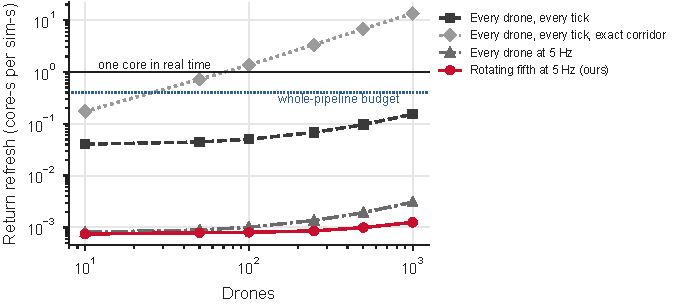
\includegraphics[width=0.86\textwidth]{figures/pdf/m4_coupling_cost.pdf}
\caption{F4, cost of coupling. CPU time to keep every drone's return plan current, per simulated second, on one core;
median of three runs. Exact corridor queries every tick exceed a full core beyond about 70 drones; the runtime's
rotating 5\,Hz schedule (Sect.~\ref{sec:design:runtime}) stays near one core-millisecond per simulated second}
\label{fig:m4}
\end{figure}
